% Chapter Template

\chapter{Background Information} % Main chapter title

\label{Chapter2} % Change X to a consecutive number; for referencing this chapter elsewhere, use \ref{ChapterX}

%----------------------------------------------------------------------------------------
%	SECTION 1
%----------------------------------------------------------------------------------------

\section{Introduction}

According to [1] Game theory is a mathematical tool and conceptual 
framework that can be used to study complex, self-interested 
interactions among rational players. A simpler explanation is that 
Game theory is the science of decision making. It originated in the 
minds of great economists like Von Nuemann and Morgeston as early as 
the 1940's as a way to explain the behaviour economics. It was then 
further developed to be used in financial markets. The theory really 
thrived in the 1950's when John Nash published several works around 
non-cooperative Games that where applied more broadly. Unfortunately 
in later years the discovery that a well-defined value system must be
first defined before expecting the solutions dervied through Game theory 
to actually be accurate accoring to [1]. The varying nature of human value systems 
prevented significant in-roads in areas where human players where 
considered, but it did not stop the application to various fields 
with defined constraints such as control-loops, war-fare, ecology, etc..[1]

There are many definitions for what a *game* is in Game theory, but lets 
consider the definition proposed by [2] where they state that a game is 
any situation involving more than one individual, each of which can make 
more than one action, such that the outcome to each individual, called 
the \textit{payoff}, is influenced by their own action, and the choice of action 
of at least one other individual. In other words a situation where rational 
agents take actions according to a strategy to maximize their own utility. 
Many situations can be arranged in this way to solve complex systems 
involving many decisions. [2]

A way to think of what is meant by \textit{strategy} in Game theory lets 
consider the analogy proposed by [19] by imagining you where playing 
a game of chess. The caveot is that you are playing via a representative, 
so in order to play the game you must create a set of instructions for 
every possible circumstance that may arise during the game. That means 
for the first move they make you must design outline the response for 
every reaction of the opponents move. The entire set of these decisions 
all the way until the end-game is a strategy for the player. 
A deterministic game like chess can be mapped out this way (even 
if it would be a very tedious excercise). These types of games are 
called finite because tehre are a limited number of moves. They are 
also considered a zero-sum game because one players gain equals 
the other players loss. Also, this game can be considered a 
compettitive game or a \textit{Non-Cooperative} game because both players 
are competing to increase their own utility at the expense of the other.

Game theory can be categorised into three main branches: \textit{Non-Cooperative} 
game theory, as mentioned above, \textit{Cooperative} game theory (coalitional 
game theory) and relatively recent branch called \textit{Evolutionary} game 
theory (EGT). The contributions to game theory can be found in Figure 1. 
as presented in [3], it shows cooperative game theory was founded by 
Neumann and Morgenstern [10], and then non-cooperative game was represented 
by Nash’s work [11],[12],[13],[14]. 

John Nash proved the existence of non-cooperative game solution, that is,
the existence of Nash equilibrium (further explained later), thus laying
the theoretical foundation of the modern non-cooperative game. Non-cooperative 
game theory essentially studies the settings where multiple payoff-maximising 
players, who have partially or totally contradictory interests over the 
system and/or personal outcomes, interact with each other. 

Cooperative games are based on the Shapley value, a value that calculates 
the \textit{fair} payoff of a player in a coalition of players. In a cooperative 
game all players are aware of the strategies chosen by other players. 
The goal in a cooperative game is to maximize the reward of all players 
involved. An example would be a group of homes with energy storage 
capacity and roof-top solar power generation working together to 
maximize overall revenue by selling energy at peak demand and meeting 
dynamic loads between them. 

As for the evolutionary game, it is generally recognized that it was 
officially founded by Maynard Smith and Price [15]. This theory can be 
regarded as an organic combination of general game theory and dynamic 
evolution process [16]. Among these, the former focuses on the game 
problem within the framework of \textit{bounded rationality} rather than 
\textit{complete rationality}, while the latter draws on the biological 
evolution theory in biology field. In short, the decision-making 
stakeholders (i.e., playersor participants) in an evolutionary game 
constantly adjust their own strategies according to environmental 
changes and the strategies of other decision-making stakeholders in 
order to adapt to the game environment under the conditions of limited 
knowledge, information and reasoning ability [9], [17].

In conclusion Game theory has evolved from combinatorial analysis of 
decision making in economics, to an encompassing theory that can apply
to acting on complex strategies in various disciplines. A game consists
of rational agents called players, a set of decisions called strategies, 
and payoff's that maximize the players utility in some way. The major 
branches of Game theory are cooperative, non-cooperative and evolutionary.
Each branch addresses various kinds of games found in nature and in 
many different disciplines. In the following section we explain the 
element sof a game in greater detail. The chapter will then continue to 
review the details of each branch of game theory and provide examples to 
illustrate the approaches.


\begin{figure}
    \centering
    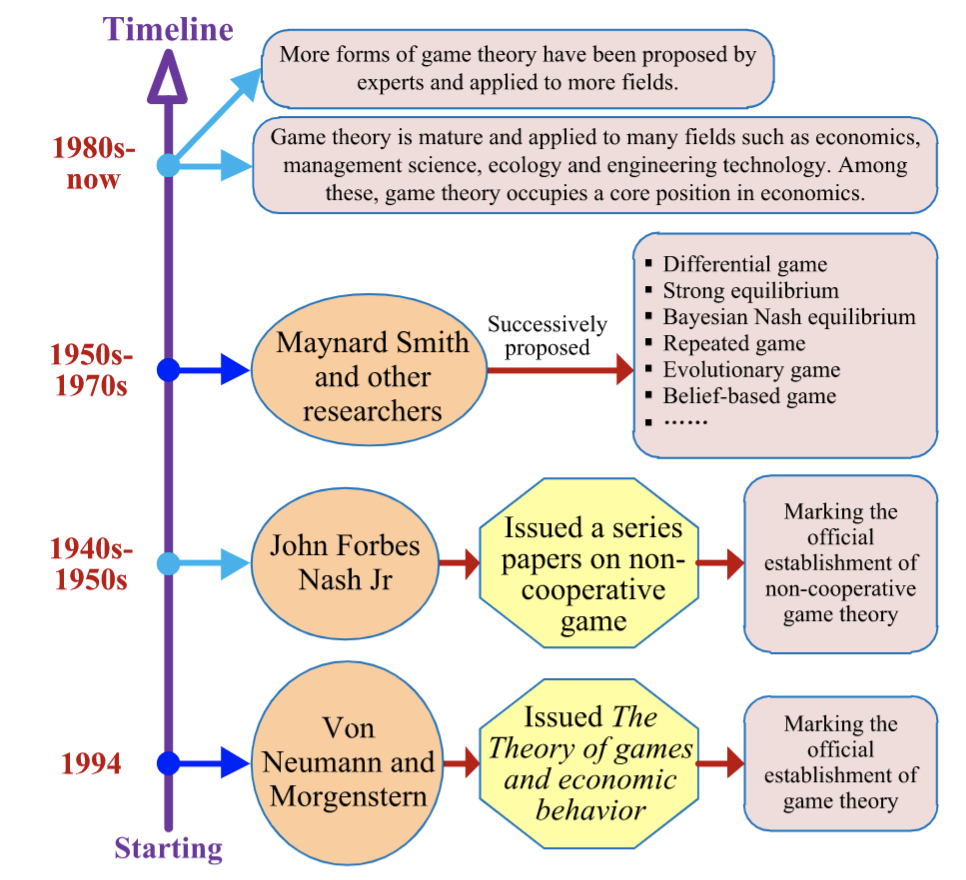
\includegraphics[width=3.0in]{Figures/timeline_gt.png}
    \caption{Evolution of Game Theory}
    \label{evolution of gametheory}
\end{figure}

\begin{figure}
  \centering
  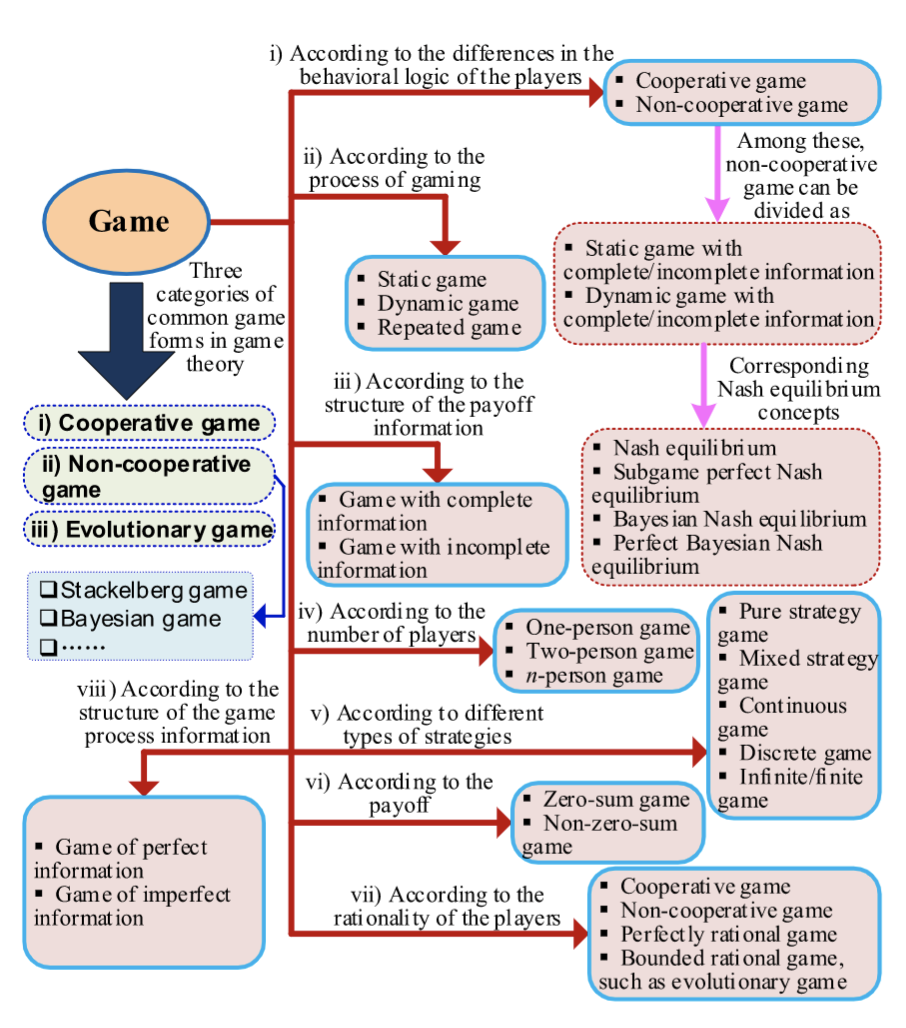
\includegraphics[width=3.0in]{Figures/game_classification.png}
  \caption{Classification of Game Theory}
  \label{classification of gametheory}
\end{figure}

\section{Elements of Game Theory}

\subsection{Pay-Off Matrix}

In an \textit{n}-player game, the goal of the participants is 
usually to minimize payments or maximize incomes. Based on this, 
a typical \textit{n}-player game [9] can be expressed as

$$G = [N;S_{1},S_{2},...,S_{n};u_{1},u_{2},...,u_{n}]$$ (1)

Where the game is \textit{G}, and \textit{N} represents a set of players 
in the \textit{n}-player game. The \textit{S} series represents the strategies 
of each \textit{n}-player. Finally the \textit{u} represents the payment for 
each \textit{n}-player. 

\subsection{Pay-Off Matrix}
The normal-form representation for the standard game model is 
the pay-off matrix as described by [2]. Each column and row represents 
the associated payoffs for each strategy as a combination of the two 
players. Given a strategy 'A' and a strategy 'B' a matrix of the game 
can be drawn to represent the responses of Player1's (P1) decision of 
strategy A and B while Player 2 (P2) chooses either A or B. The value
at each cell then represents the reward/loss of the decision for each 
player. 

\subsection{Pay-Off Matrix Example}

A good example to illustrate the pay-off matrix is to consider
the idea of stop lights in a busy intersection. Both drivers can be 
considered as players in this game and the decisions they can take 
(stop,go) can be expressed in a combinatory manner using the normal-form 
representation. 

The rewards for the game can be arbitrarily 
estimated given the desire of either players. If both players 
decide to "Go" at the same time then they will end up in a 
collision. This does not benefit either player so we place the 
reward for each accordingly (-5,-5). If either of the drivers 
have to stop to let the other go then the player who is stopped 
is inconvenience (reward of 0), while the driver who was able 
to go is now on its way and happy (reward of 1). The final strategy 
is if both players are stopped and niether move forward wasting 
time but not in a collision so not as bad but still a loss 
(reward of -1).

\begin{figure}[th]
  \centering
  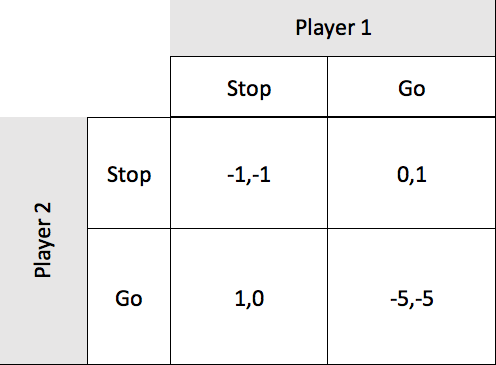
\includegraphics[width=3.0in]{Figures/pay-off-matrix.png}
  \decoRule
  \caption[2 player-payoff]{Pay-off matrix for 2 players.}
  \label{fig:Pay-offMatrixfor2Players}
\end{figure}


\begin{figure}[th]
  \centering
  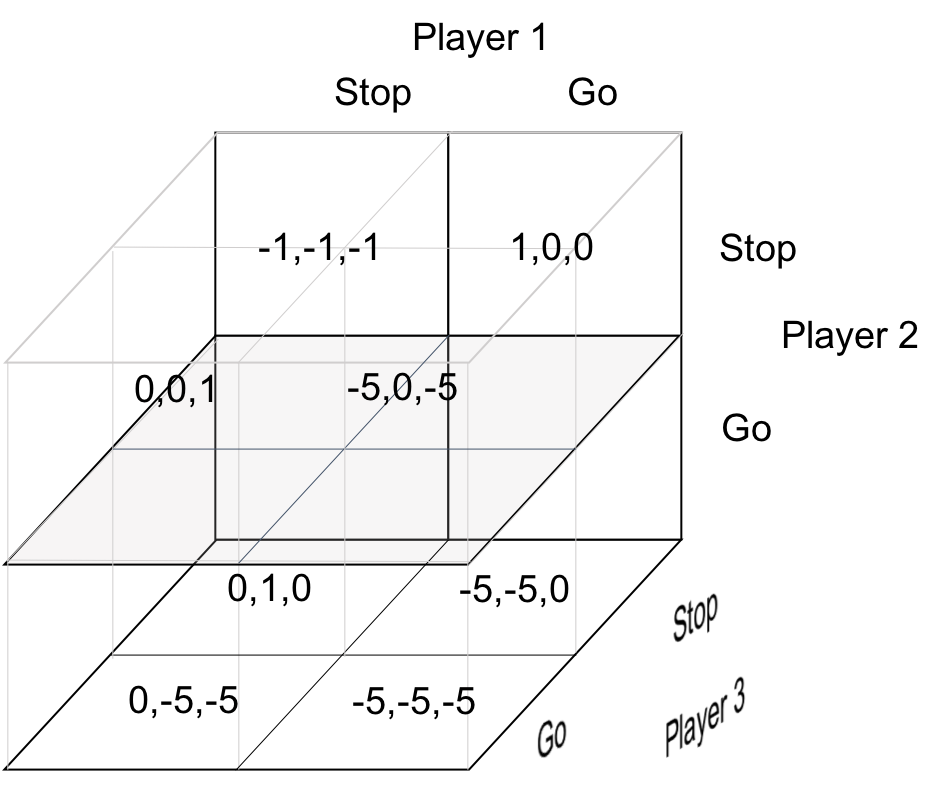
\includegraphics[width=3.0in]{Figures/3way_intersection}
  \decoRule
  \caption[3 player-payoff]{Pay-off matrix for 3 players.}
  \label{fig:Pay-offMatrixfor3Players}
\end{figure}


The possible decisions of the players in the game are
mapped out in the game matrix. The strategy for each player 
can now be assesed. The goal would be to find the best strategies
for player 1 and for player 2 respectively. For player 1, 
the strategy where he is able to go is when player 2 must stop
(1,0). The best strategy for player 2 is the opposite (0,1).
Since there are no better moves for each player to take these 
are both known as Nash Equilibriums. The equilibrium of a non-cooperative
game is when either player has no other decisions available that 
would better thier individual positions. There can be more than 
one nash equilibrium in a game .

\subsection{Components of a Game}

1) Players/Participants :  The  participants  in  the  game  who  
can  decide  their  own  strategies.  An  important  assumption  
is  that  the  players are rational, which means that they don’t 
leave things to chance and don’t take advantage of others’ mistakes. 
If we assume rational agents that have all rationality and all relevant 
information then the agent can model the game as an optimization problem. 
Unfortunately people do not always choose the most rational choice in 
real life. This then reduces the accuracy of classical game theory. 
Optimization is not just a single value system but many that also 
optmizes accross social and cultural systems.[1]

2) Strategy : A collection of all the strategies available for all 
players. According to whether a player’s strategies are finite, we can 
divide games into three groups: *finite games* and *infinite games*. 
Sometimes a strategy set can be infinite since it can by almost any option,
or only 3 for example in the game of rock, papers, scissors. There are
some strategies that do not involve randomness (finite strategy) such 
as to tic-tac-toe.finite games are also known as *matrix  games*. An  
*infinite  game*  is  said  to  be  a *continuous-kernel*  game if  
the  action  sets  of the players are continua, and the players’ 
objective functions are continuous with respect to action variables 
of all players.[5]

3) Pay-offs/Payment: After each player in the game chooses a  strategy
from  their  own  strategies  set,  a  relevant  result  
(a  group of data) is provided to show each player’s gain or loss.
A good payoff is the fundamental goal of a player, and is the main
basis of a player’s judgment and behavior. Pay-offs are also known
as the players preferences described as 'utility' and must be 
understood clearly for the model to be effective. The payoffs are
very subjective. If there is a ranking to the payoff it is called 
\textit{ordinal} , if it is just a subjective quantity value then it is 
a \textit{cardinal} payoff.[1]

Honorable mention, \textit{Order} , technically an overlooked aspect of 
games is the order in which players make a decision. 

4) Orders:  When  different  players  are  about  to  decide,  
there is a need to decide the orders. Sometimes players make 
their decisions at the same time to make sure that the game is fair;  
sometimes  players  make  decisions  one  after  another;  most times 
in reality players may choose their strategies more than once.  
Different orders result in quite different situations.

\section{Cooperative Games}

\subsection{Shapley}
Write your subsection text here.

\section{Non-Cooperative Games}

\subsection{Non-Cooperative Game Models}

The different types of models as defined in [4] consists of the following:

1) Ordinary Non-Cooperative game: Analyze the problem and abstract the players,
strategies and the pay-offs for the model. The properties of the model should 
result in equilibrium solutions that could solve the problem.

2) Generalized Nash equilibrium game: Each  player’s  decision affects 
not only other players’ payoffs, but also their feasible strategies set.

3) Cournot game: Derived from prisoner's dilemma model. Models the pay off  
capable in a game when both players will need to implement the strategy at the
same time. Used in behavioral economics to determine pay-off of individual decisions.

4) Stackelberg game: Similar to the Cournot game, but assumes that there is a 
player that is a leader (goes first) and a player that goes after (follower).
The model has the leader anticipate the followers response and include that 
in its own response. This technique helps the leader to optimize its utility
in a market shared among two players.

5) Bounded rationality game: Models that attempt to remove the assumption
that players are completely rational. Considering that players can take
actions that do not immediately benefit them can possibly model the 
uncertainty of initial value assumptions of the utility modeled for each player.

6) Repeated game: A series of basic games one after the other. This type of 
model shows the varied results capable given the strategies implemented in 
each instance of a game.

\subsection{Stackelberg Model Simulation}
A Stackelberg Game is a type of noncooperative game that deals with a 
multi-level decision making process of a number of independent decision 
makers or players(followers) in response to the decisiont taken by a 
leading player (the leader).

The game has the following components:

a) Followers in the game that respond to a price set by the leader

b) The strategy of each of the followers in terms of satisfying 
some constraint.

c) The utility function of each follower that captures the benefit 
of consuming the demand.

d) The utility function of the leader which captures the total profit.

e) The price per unit quantity

The utility function of the follower represents the level of 
satisfaction of the follower. It is a function of the profit it recieves. 
The utility function is non-decreasing because each follower is 
interested in maximizing its profit. The marginal benefit of the 
follower is also considered a non-increasing function. The marginal 
benefit gets saturated the closer it gets to the maximum profit. 
The utility of a follower decreases as the price of a unit or cost 
of meeting a demand increases .

If the constraint is the same for all players then this gives rise to 
a noncooperative resource sharing game between the followers. A game l
ike this represents a jointly convex generalized Nash equilibrium 
problem (GNDP) due to the same shared constraint. In game theory the 
coupling of the constraints has solution called the Gneralized Nash 
Equilibirum(GNE).[3]

The stackleberg duoply is a non-cooperative game between two players 
where one is a leader and the other is a follower. They are the only 
two players able to supply the needs of the market by creating some 
quantity of goods. Each player has a utility function that will be 
satisfied if they can maximize the profit of supply a quantity of 
goods to the demand curve of the market considering the cost to provide 
a unit of goods.  [5],[7]

Define a pricing demand as a linear function and call it a 
"Market Demand Curve"

```
P = a  -  b * Q
```

Where Q is the market quantity demanded and P is the market price in dollars
The firms create the quantity.

The quantity created for the market comes from multiple firms. 
The firms in a Stackleberg game provide some quantity after the 
leader firm goes first. The leader firm assumes the moves of the 
other firms and tries to maximize its profit by incurring the costs 
to meet the demand that it deems appropriate given its own costs. 
The demand is met through a total quantity that can be represented 
by the combination of all of the players quantity. 

```
Q = q1 + q2 + ... qN
```

The cost to meet a single unit of demand per unit qunatity created. 
This is a pre-defined metric or can be a dynamic value. Knowing the 
marginal costs is critical to determining the other players moves. 
The Leader needs to know what it would cost other players to take action.

Begin backward induction to determine what the reaction would be of 
the other firms. Lets assume two firms A, and B. The procedure to 
determine the Leaders (firm A) move would be as follows:

1. Calculate Firm B's reaction
2. Calculate Firm A's response to B's reaction
3. Implement Firm A's response
4. Calculate Firm B's response given A's response
5. End Game

$$ N_{firms} = 2$$ (2)
$$ MC_{a} = 10$$ (3)
$$ MC_{b} = 12$$ (4)
$$ P_{T} = -Q_{d}m+b$$ (5)
$$ P_{T} = -Q_{d}*0.5+120$$ (6)

By inspecting the demand curve we can see that all the quantity 
generated by the payers (x-axis) will result in a total price for 
all the quantity (y-axis) at different levels of demand met. 
The pricing demand curve can now be used as a total demand and 
total quantity output that will be presented to the players. 
At some break even point the price demand for a unit is no longer 
advantageous considering the cost to the player to meet that demand.

The break even point would be the profit maximizing point for the player. 
In the stackleberg game the leader tries to maximize its output by 
looking at the break even point of the secondary player. If the 
marginal costs are lower for the follower they can generate more 
quantity and outsell the leader. This means the leader should make
enough to break even and just enough to reduce the gains of the follower.

Again, by only looking at the demand curve the leader can only 
determine a break even point based on its own cost. As soon as 
it costs more to meet the demand than the price of the demand 
then the leader stops and no longer produces. If the demand must be met, 
then the rest of the demand is left for the second player to take on. 
If the second player looks at the remaining demand and only supplies 
what it can break even then both players are left supplying demand 
with diminishing returns.

To avoid having to supply diminishing returns the leader can take 
into account the maximizing move for the second player and then 
include that in determining its stake in the market based on its 
own costs and break even point.

Total Market Quantity Demand:
$$ Q_{d}= q_{a} + q_{b}$$(7)

Market Demand Curve:

$$ -0.5*Q_{d} + 120 = -0.5*q_{a} + -0.5*q_{b} + 120$$(8)

$$TR_{b} = -0.5*q_{a}*q_{b} - 0.5*q_{b}^2 + 120*q_{b}$$(9)

Marginal revenue can be derived from the derivative of the total 
revenue equation (9), with respect to the firm.

$$ MR_{b} = \frac{\partial d}{\partial q_{b}}(-0.5*q_{a}*q_{b} - 0.5*q_{b}^2 + 120*q_{b})$$ (10)
$$ MR_{b} = -0.5*q_{a} - q_{b} + 120$$ (11)

The reaction of the follower can be estimated by the leader by 
solving when the marginal cost of the follower will equal the 
marginal revenue of the follower. Setting them equal and solving 
for the quantity in terms of the quantity provided by the leader 
firm A we get the following reactionary quantity for firm B.

$$ q_{b}^* = -0.5*q_{a} + 108$$ (12)

The leader takes into account all the reactions and creates a 
leader response to the reactions. The approach is to use back 
induction to take the forecasted reaction of the follower when 
the marginal cost is equal to the marginal revenue (profit maximizing). 
That means that the follower will stop at some break even point 
that maximizes its profits. Given that information the leader can 
take that reaction and assume it is what the follower will do. 
The assumption is used in the price demand formula. By substituting 
equation (12) into equation (8) the demand for the leader is now 
shown below in (13). Knowing the demand the total revenue and 
marginal revenue can also be inferred.

$$ P_{leader} = -0.25*q_{a} + 66$$ (13)
$$ TR_{a} = -0.25*q_{a}^2 + 66*q_{a}$$ (14)
$$ MR_{a} = \frac{\partial d}{\partial q_{a}}(-0.25*q_{a}^2 + 66*q_{a})$$ (15)
$$ MR_{a} = -0.5*q_{a} + 66$$ (16)

The last step in the backwards induction for the leader is to try to 
maximize his profit by only providing a quantity where the followers 
quantity has been considered in the game. The final quantity to be 
implemented by the leader is done just as before by setting marginal 
revenue equal to marginal cost and finding quantity.

$$ q_{a}^Final = 112$$ (17)

If we implement the leaders quantity output and then recalculate 
the resulting quantity for the follower, the follower will have a 
different output than what was orginally measured by the leader 
since the leader has now taken its maximum demand.

$$ q_{b}^Final = 52$$ (18)
